%
%   MIX - Userreference
%

\documentclass[a4paper,12pt]{article}

\setlength{\textwidth}{170mm}
\setlength{\textheight}{255mm}
\setlength{\oddsidemargin}{-5mm}
\setlength{\topmargin}{-18mm}


%\usepackage[OT2]{fontenc}
\usepackage[latin1]{inputenc}
\usepackage{supertabular}
%\usepackage{epsfig}
\usepackage{graphicx}
\usepackage{xr}

\fontencoding{T1}
\fontfamily{garamond}
\fontseries{cmtt}
%\fontshape{it}
%\fontsize{12}{15}
\selectfont

%\usepackage{aaai}
%\usepackage{times}

\title{MIX - Micronas Interconnect Specification Expander}
\author{Userreference}
\date{6.10.2003}

\begin{document}

%\begin{titlepage}
%\begin{tabular}{p{20mm}l}
%\multicolumn{2}{r}{\bf {MIX} - Micronas Interconnect spec. eXpander}\\[1mm]
%\hline \\[3mm]
%& MIX - \\
%& Developer\\
%& Documentation\\[5mm]
%& Micronas - Munich\\[5mm]
%\hline \\[20mm]
%\end{tabular}
%\end{titlepage}gin{titlepage}


\maketitle
\newpage

\section{MIX - Micronas Interconnect Spec expander}
\section{Introduction}
\section{Management Summary}
\tableofcontents
\section{Installation}
The MIX toolset uses the Perl scripting language. Please install a recent version of Perl on your workstation, e.g. the freely available ActiveState Perl  from K:$\backslash$PROJECTS$\backslash$MIX$\backslash$PROG$\backslash$ActivePerl-5.6.1.633-MSWin32-x86.msi. Apart from that no installation is required.\newline
Start MIX from the network drive like described in the examples below. That will also make sure, that you are using the most recent release automatically.
After the Perl installation, you can run MIX. immediately. Open a command shell on your desktop workstation:\newline
\hspace*{15mm}\begin{math} Start \longrightarrow Run \longrightarrow cmd\end{math}\newline
and type:\newline
\hspace*{15mm}K:$\backslash$Projects$\backslash$MIX$\backslash$PROG$\backslash$mix\_0.pl foo.xls\newline
Caveat: Currently MIX is available on MS-Windows, only!\newline

\section{Getting Started}
To receive useful results, MIX reads in various input spreadsheet data. At least you will need to prepare a description of your design hierarchy (\begin{bf}HIER\end{bf}) and the connectivity sheet (\begin{bf}CONN\end{bf}). Optionally MIX will convert a input/output sheet IO, listing input/output pads and iocells and how these are linked to the core logic into appropriate hierarchy and connection lists.

\subsection{A simple example}
To understand the usage of the various tables and options, a very simple example is shown and extended step by step. The simple example just has two components \begin{it}a\end{it} and \begin{it}b\end{it}, which are connected by the signal \begin{it}sigfoo\end{it}. The two instances have a common parent \begin{it}chip\end{it}.\\
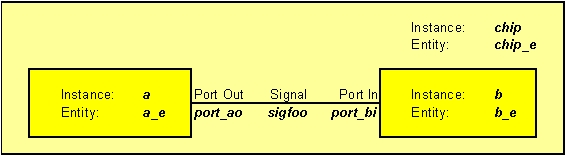
\includegraphics[scale=0.9]{images/mix_simple_0.jpg}\\
Image 1: mix\_simple.xls\newline
\newline
The equivalent description of this simple design in MIX is made up from a worksheet \begin{bf}HIER\end{bf}.\\
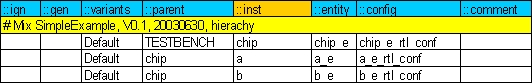
\includegraphics[scale=0.8]{images/mix_simple_1.jpg}\\
The first row defines the table headers names. The names have to be in the form "::NAME". Several of the columns are required, some are optional and you can define additional columns on your own. For HIER sheets the "::inst" column is the primary key. One design element will be generated for each new name of an ::inst row. If a name is defined several times, these lines will be overloaded or summarized, depending on built-in rules of the MIX converter.\newline
The "::ign" column has to come first. If it starts with a \#, the rest of this row will be ignored. All other columns can be added in arbitrary order.\newline
\newline
The second required worksheet is \begin{bf}CONN\end{bf}:\\
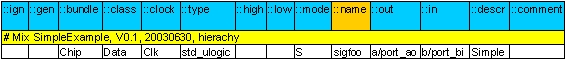
\includegraphics[scale=0.8]{images/mix_simple_2.jpg}\\
As you see, this worksheet also starts with the table header definition line. The primary field is the "::name" column. The "::in" and "::out" columns are used to define the drivers and loads for the signals.

\subsection{Mix it!}
Run the MIX converter tool in the directory the excel spread sheet is stored in:\newline
\begin{tt}\hspace*{15mm}\$ cd $\backslash$work$\backslash$MIX$\backslash$doc$\backslash$parts$\backslash$simple\newline
\hspace*{15mm}\$ K:$\backslash$Projects$\backslash$MIX$\backslash$PROG$\backslash$mix\_0.pl mix\_simple.xls\end{tt}\newline
This reads in the design description and evaluates the various sheets. It creates output files with an intermediate excel design description (\begin{tt}mix\_simple-mixed.xls\end{tt}) and the same data in a internal format (\begin{tt}mix\_simple.pld\end{tt}). A log file (\begin{tt}mix\_0.pl.log\end{tt}) and the HDL output files are written in the same run. Image 2 shows a screenshot of the \begin{tt}mix\_simpe.xls\end{tt} conversion. Only the most important errors and warnings are written to the screen, while a lot of information will be written to the log file. Search for the keywords "ERROR" and "WARNING" to verify proper conversion.\\
\\
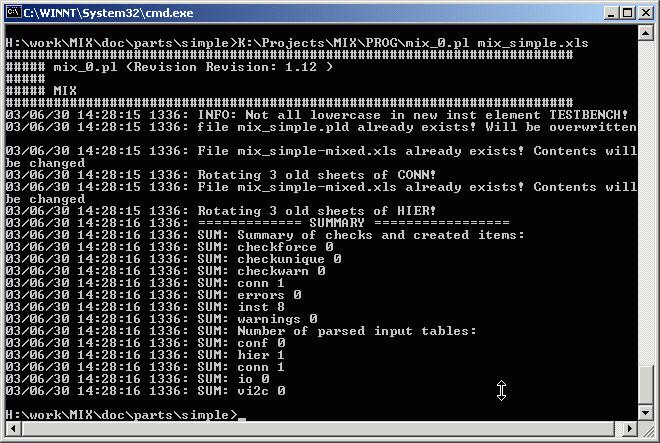
\includegraphics[scale=0.6]{images/mix_simple_cmd.jpg}\\
Image 2: mix\_simple conversion\newline
All output files are stored in the current working directory. Old versions of the output files are overwritten. Except the log file that is appended by each converter run. The intermediate excel description file keeps a history of previous HIER and CONN sheets by rotating \_N extended worksheet names.\\
\\
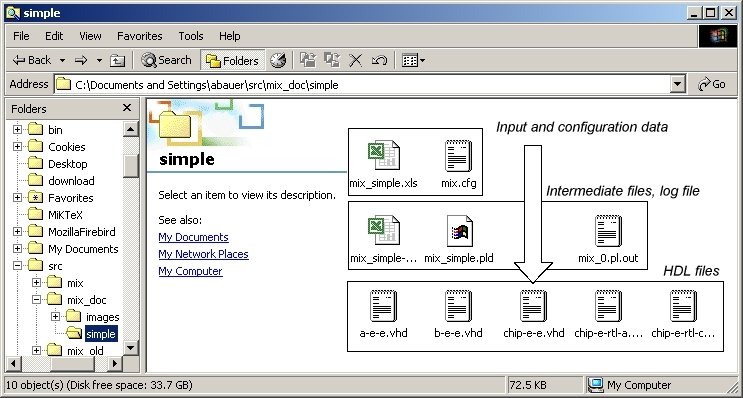
\includegraphics[scale=0.6]{images/mix_files.jpg}\\

\subsubsection{You get what you typed}
MIX generates various HDL files defined by the input data. If you select VHDL (also the default language) as output description for a hierarchy element, each element results in an appropriate entity, architecture and configuration description. By default MIX writes one file for all entities, one for all architecture and one for all configuration descriptions. Those file names are derived from the last excel input file name by stripping of the .xls extension and attaching a -e.vhd, -a.vhd and -c.vhd.\newline
Here the working directory of the simple example contains a file mix.cfg, which is the convenient storage for MIX run-time configuration options. The lines "MIXCFG outarch ARCH", "MIXCFG outenty ENTY", and "MIXCFG outconf CONF" switch MIX outputs to separate files for each entity, architecture and configuration. In this case the file names are defined by the element name:
\begin{table}[htb]\begin{tabular}{|p{3cm}|p{4cm}|p{3cm}|p{5cm}|}\hline
\begin{bf}Type\end{bf}&\begin{bf}Basename\end{bf}&\begin{bf}Extension\end{bf}&\begin{bf}Example\end{bf}\\\hline
Entity & ::entity-column & -e.vhd & chip\_e-e.vhd \\\hline
Architecture & ::entity-column & -rtl-a.vhd & chip\_e-rtl-a.vhd \\\hline
Configuration & ::entity-column & -c.vhd & chip\_e-rtl-conf-c.vhd\\\hline
\end{tabular}\caption{``\_'' in the filenames extension are converted to ``-''}\end{table}\newline
By default MIX does not write output data for leaf blocks (instances which are not parent for other instances). Adding a line like "MIXCFG generate.output.arch leaf" into the mix.cfg file changes that.\newline
The generated output files contain head, body and footer sections. See the screenshots of the file a-e-e.vhd and chip-e-rtl-a.vhd for examples of an entity and an architecture definition.\\
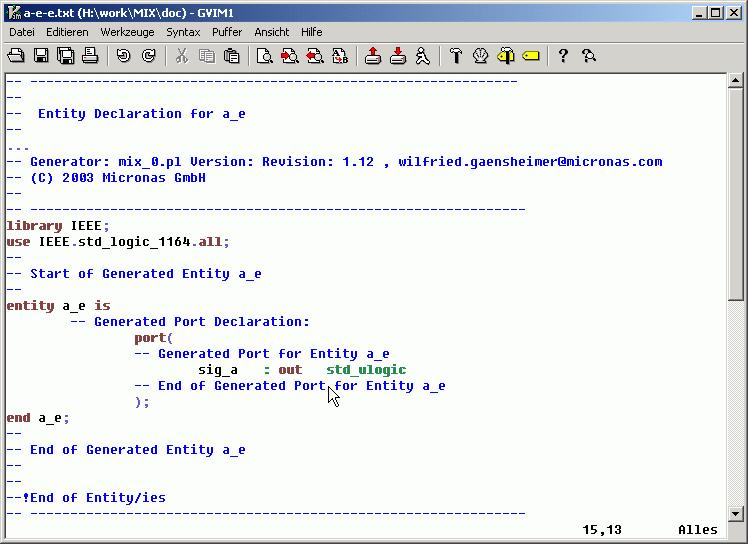
\includegraphics[scale=0.55]{images/mix_a-e-e.jpg}\\
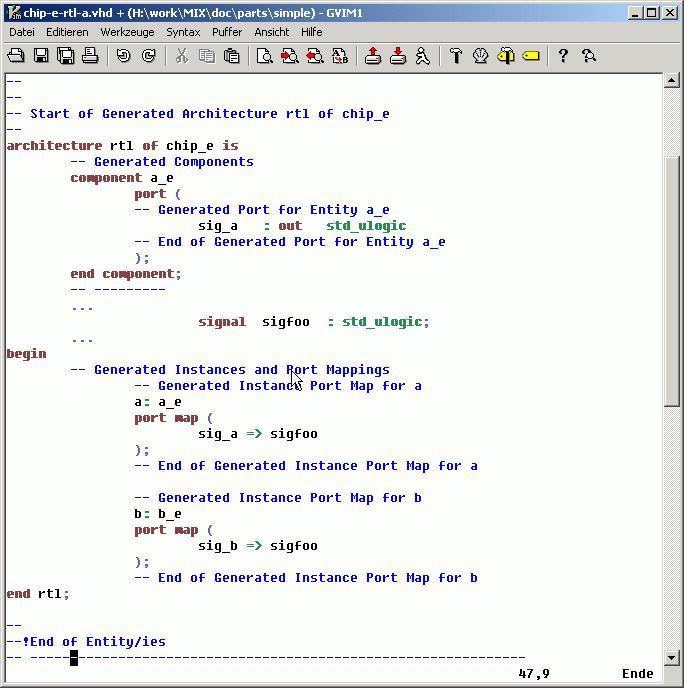
\includegraphics[scale=0.6]{images/mix_chip-e-rtl-a.jpg}\\

\section{Details}
\subsection{Initialization with -init}
You can use the -init command line option to create the needed files:\newline
\hspace*{20mm}\begin{tt}\$ mix\_0.pl -init foo.vhd bar.xls\end{tt}\newline
will create the file \begin{tt}bar.xls\end{tt}, which has the following three worksheet categories:\newline
\hspace*{10mm}- empty HIER, CONN and IO sheets\newline
\hspace*{10mm}- template sheets with numerous examples TMPL\_(HIER|CONN|IO)\newline
\hspace*{10mm}- import sheets IMP\_HIER and IMP\_CONN (only of more *.vhd or
\newline\hspace*{11mm} *.v files are given as command line arguments).\newline
You will also get a \begin{tt}mix.cfg\end{tt} file. If \begin{tt}bar.xls\end{tt} or \begin{tt}mix.cfg\end{tt} already exists, the command will exit without changes. The import of \begin{tt}*.vhd\end{tt} and \begin{tt}*.v\end{tt} files is experimental and meant to give a way of getting a start description of your design. In case of VHDL files, only entity descriptions are imported. Take care of getting signal names and instance names properly.

\subsection{Common worksheet properties}
All worksheets parsed by MIX share some common properties.
There needs to be a header line consisting only of keywords with leading double colon. All data before the header line is ignored. Only the first header line will be evaluated. Data in columns with no header or malformed headers will be ignored.\newline
Commonly understood table headings are \begin{tt}::ign\end{tt} and \begin{tt}::comment\end{tt}. The \begin{tt}::ign\end{tt} column is special, because it needs to be the first column of a sheet. If a cell in the \begin{tt}::ign\end{tt} column starts with a \begin{tt}\#\end{tt} or a \begin{tt}//\end{tt}, the complete row is ignored.The \begin{tt}::comment\end{tt} column can contain user or program generated comments for a given row. It's data will be appended to it's contents as it appears.\newline
MIX reads the cell values. This is, for Excel and Star(/Open)-Office, what you see , not the real contents of the cells. Thus all formulas can be used to define the cell values (note: csv is not able to do that).\newline
A lot of predefined text macros are understood and converted by MIX. A text macro is made up by a name surrounded by \begin{tt}\%\end{tt} signs. Retrieve a complete list of macros with the -listconf command line switch and grep all lines starting with "\begin{tt}MIXCFG macro\end{tt}". The table \begin{tt}\%macro\%\end{tt} gives a list of predefined macros, their default settings and wether this macro can be used by the user. You can use text macros inside of any cell.\\
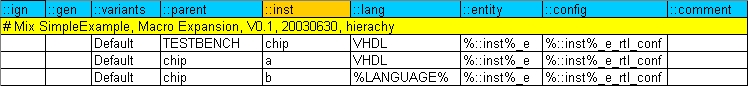
\includegraphics[scale=0.6]{images/mix_table0.jpg}\\
A second type of macros are available to reference other columns of a like through \begin{tt}\%::NAME\%\end{tt}. This will be replaced by the contents of the \begin{tt}::NAME\end{tt} column of this row. \begin{tt}::NAME\end{tt} has to be defined for the current worksheet, obviously. In the above example \begin{tt}\%::inst\%\_e\end{tt} will evaluate to \begin{tt}chip\_e\end{tt}, \begin{tt}a\_e\end{tt} and \begin{tt}b\_e\end{tt} accordingly. \begin{tt}\%LANGUAGE\%\end{tt} becomes vhdl. Macro expansion happens just before the intermediate design data is written out, after evaluation of all input data. Recursive macro expansion is not implemented. Macros in primary keys like signal and instance names are evaluated at signal or instance creation time.

\subsection{Special Spreadsheet-format properties}
MIX is able to read three different table formats: csv(Comma-Seperated-Values), sxc(Star-Office-Spreadsheet) and xls(Excel-Spreadsheet). While Excel and StarOffice Spreadsheets are full featured, the csv Format does not understand formulas. This is because the real content and it's values are same in csv. The only colored output can(at this moment) be achieved by writing Excel-Spreadsheets(for this an already installed Excel is needed). While writing Excel-sheets implies Windows, reading input can be done on every Platform(if it got a Perl port). Trying to read a Excel-Sheet on non-Windows grounds will cause MIX to produce csv per default. The output format can be forced by setting \begin{tt}format.out\end{tt} to \begin{tt}csv\end{tt}, \begin{tt}sxc\end{tt} or \begin{tt}xls\end{tt}. In this case MIX will read the given input file and produce the forced output format.

\subsection{HIER sheet properties}
The hierarchy of a design is defined in the HIER sheet. By default the HIER sheet is named HIER, but you can set the configuration value \begin{bf}hier.xls\end{bf} to a Perl regular expression. MIX will then consider all worksheets which names match the perl regular expression, to be HIER definitions. In that case you are free to use different header definitions on different sheets.\newline
The HIER sheets require at least the columns marked man. (mandatory) in the following table.

\begin{table}[htb]\begin{tabular}{|l|p{4cm}|p{4cm}|p{15mm}|p{2cm}|}\hline
\begin{bf}Column name\end{bf} & \begin{bf}Descriptionend\end{bf} & \begin{bf}Default value\end{bf} & \begin{bf}Req.\end{bf} & \begin{bf}Example\end{bf}\\\hline
::ign & Ignore line & $<$empty$>$ & man. & \# comm. \\\hline
::gen &  Generator and match & $<$empty$>$ & man. & see below \\\hline
::variants & Variant selector & Default & opt. & Var1\\\hline
::parent & Instance name of this instances parent cell & W\_NO\_PARENT & man. & chip \\\hline
::inst & Instance name, primary key! & n/a & man. & a\_i1\\\hline
::lang & Language definition & VHDL & opt. & vhdl \\\hline
::entity & Entity name & W\_NO\_ENTITY & man. & a \\\hline
::config & Configuration name & W\_NO\_CONFIG & man. & a\_rtl\_conf \\\hline
::shortname & Short name & $<$empty$>$ & opt. & text \\\hline
::use & Additional, project specific libraries & $<$empty$>$ & opt. & padlib.foo \\\hline
::comment & Comment field & $<$empty$>$ & opt. & text \\\hline
\end{tabular}\end{table}

Internally the kewords \begin{tt}::debug\end{tt}, \begin{tt}::hierarchy\end{tt}, \begin{tt}::skip\end{tt} and \begin{tt}::default\end{tt} are used. Please do not use them. Apart from that you are free to add columns of your own. User defined columns are usable in \begin{tt}\%::NAME\%\end{tt} macro expansion and are listed in the intermediate design data output.\newline
Only the \begin{tt}::inst\end{tt} column has to contain a value in each row (which could be a \begin{tt}\%::NAME\%\end{tt} macro, though). All other columns will receive more or less reasonable default values in case they are left empty.

\subsection{HIER columns details}
\begin{bf}::gen\end{bf}\hspace*{12mm}If a cell here is not empty, the line will be considered as\newline\hspace*{18mm} generator. See description of generator statements below.\newline
\begin{bf}::variants\end{bf}\hspace*{6mm}Select a line depending on the -variant command line switch. If
\newline\hspace*{18mm}-variant VAR is set, only lines whose \begin{tt}::variant\end{tt} cell contains the keyword
\newline\hspace*{18mm}VAR, Default or empty, are selected and read in. Several variants may be
\newline\hspace*{18mm}given in one cell, separated by ",". Without specifying the \begin{tt}-variant\end{tt} switch,
\newline\hspace*{18mm}the "Default" and empty \begin{tt}::variant\end{tt} cells are read in and evaluated.\newline
\begin{bf}::inst\end{bf}\hspace*{10mm}Defines the instance name. If the same name appears in several rows, the
\newline\hspace*{18mm}resulting row will be overloaded from all input rows. The exact behaviour
\newline\hspace*{18mm}depends on the column name. Some are concatenated, some are replaced.\newline
\begin{bf}::lang\end{bf}\hspace*{9mm}HDL language selection, case insensitive. If this column is omitted or empty,
\newline\hspace*{18mm}VHDL output is generated. The default value can be changed by means
\newline\hspace*{18mm}of the macro.\%LANGUAGE\% macro. Currently only VHDL and\newline\hspace*{18mm}Verilog are supported (XXX: Verilog output still t.b.d.).\newline
\begin{bf}::config\end{bf}\hspace*{6mm}Define the configuration name. It defaults to \%DEFAULT\_CONFIG\%, which
\newline\hspace*{18mm}evaluates to \%::entity\%\_\%::arch\%\_conf. If the language of this entity is set
\newline\hspace*{18mm}to Verilog, no configuration will be printed nor will it be added to parent cell
\newline\hspace*{18mm}configurations. The keyword \%NO\_CONFIG\% will also suppress output of
\newline\hspace*{18mm}configuration for this entity.\newline
Additional columns:\newline
\begin{bf}::arch\end{bf}\hspace*{9mm}If no ::arch column is given, architecture will default to "rtl". This is defined
\newline\hspace*{18mm}by the configuration hier.field.::arch.[3] = rtl; and cannot be changed globally.\newline
\begin{bf}::use\end{bf}\hspace*{11mm}Add project specific libraries and work packages to the HDL description files.
\newline\hspace*{18mm}See the ::use details below.

\subsubsection{::use Add Project Specific Libraries}
The optional "\begin{tt}::use\end{tt}" column allows to add libraries and work packages for a entity. Several libraries can be added, separated by comma or white space. In case of VHDL output, the use statement is added to the entity declaration, only. You can override that by adding a leading \begin{tt}ALL:\end{tt}, \begin{tt}ARCH:\end{tt} or \begin{tt}CONF:\end{tt} keyword for this instance/entity. To change that globally, modify the configuration variable output.generate.use.\newline
For each given library an appropriate text sequence is added:\newline
\hspace*{20mm}\begin{tt}foo.lib\end{tt}, \begin{tt}bar.lib.something\end{tt}\newline
will be printed as\newline
\hspace*{20mm}\begin{tt}library foo;\end{tt}\newline
\hspace*{20mm}\begin{tt}use foo.lib.all;\end{tt}\newline
\hspace*{20mm}\begin{tt}library bar;\end{tt}\newline
\hspace*{20mm}\begin{tt}use bar.lib.something.all;\end{tt}\newline
If different instantiations of a entity have different ::use\newline
definitions, MIX adds up all these.\newline
To change the global default value of\newline
\hspace*{20mm}\begin{tt}library IEEE;\end{tt}\newline
\hspace*{20mm}\begin{tt}use IEEE.std\_logic\_1164.all;\end{tt}\newline
modify macro \begin{tt}\%VHDL\_USE\_DEFAULT\%\end{tt}.\newline
To add a library globally, add the appropriate text to the macro.\begin{tt}\%VHDL\_NOPROJ\%\end{tt} configuration, which will be used if no library is defined in the \begin{tt}::use\end{tt} column.\newline
A second usage is to suppress the component declaration output by the \begin{tt}\%NDC\%\end{tt} or \newline\begin{tt}\%NO\_COMPONENT\_DECLARATION\%\end{tt} keyword. This is useful for instances, whose entities are taken from libraries.\newline
\newline
Examples: see \begin{tt}t/sigport.xls\end{tt} and \begin{tt}t/sigport/use/*.vhd\end{tt} for more examples.\newline
Configuration: \begin{tt}output.generate.use = enty\end{tt}

\subsection{Special HIER sheet properties}
\begin{tt}\%TOP\%\end{tt} is a pseudo instance and used for internal purposes, only.

\subsection{CONN sheet details}
The design connections are defined in the CONN sheet. The primary key of this sheet is the signalname as given in "\begin{tt}::name\end{tt}". Signalnames are globally known for the design. All appearances of a name are connected, creating intermediate ports as needed.

\subsection{typecast}
The type of a signal can be typecasted by appending a function name with a \begin{tt}'\end{tt} to the \begin{tt}::in\end{tt} and \begin{tt}::out\end{tt} definitions.\newline
Example:\newline
\hspace*{20mm}\begin{tt}::name\end{tt}\hspace*{20mm}\begin{tt}signal\_a\end{tt}\newline
 \hspace*{20mm}\begin{tt}::type\end{tt}\hspace*{20mm}\begin{tt}type\_a\end{tt}\newline
 \hspace*{20mm}\begin{tt}::in\end{tt}\hspace*{24mm}\begin{tt}inst\_a/port\_a'typefunc\end{tt}\newline
 \hspace*{20mm}\begin{tt}::out\end{tt}\hspace*{22mm}\begin{tt}inst\_b/port\_b'typefunc\end{tt}\newline
\newline
The signal \begin{tt}signal\_a\end{tt} will be of type \begin{tt}type\_a\end{tt}, while the connecting ports of \begin{tt}inst\_a\end{tt} and \begin{tt}inst\_b\end{tt} are converted by applying the typecast function \begin{tt}typefunc\end{tt}.\newline
Caveat: typecast support is experimental.\newline

%wig20031222: top level port generation.
\subsection{Automatic Generation of Toplevel Ports}

If the signal mode as defined in the \begin{tt}::mode\end{tt} column matches one of I, O or IO, MIX will create top level ports.
This feature can be disabled by the configuration variable \begin{tt}output.generate.inout\end{tt}. Possible values are
\begin{tt}mode\end{tt}(enable top level port generation) and \begin{tt}noxfix\end{tt}(do not prefix and postfix generated port names for
top level ports), which are set by default.
To exclude some signals from automatic top-level port generation, use 
\begin{tt}output.generate.xinout sig\_foo,sig\_bar\end{tt}. This feature is usefull if you need to use internal inout signals, but do
not want to have them wired to the top-level.

\subsection{CONN columns details}

\subsection{Special CONN sheet signals}
Special signal names:\newline
\begin{tt}\%LOW\%\end{tt}, \begin{tt}\%HIGH\%\end{tt}, \begin{tt}\%LOW\_BUS\%\end{tt}, \begin{tt}\%HIGH\_BUS\%\end{tt}\newline

\subsubsection{\%OPEN\% aka. open}
Used the \begin{tt}\%OPEN\%\end{tt} signal to leave some pins of module bar port a open MIX has no knowledge about ports. Everything is defined in terms of signals and instances. Use the "\begin{tt}open\end{tt}" pseudo signal to define the extra pins.\newline
\newline
E.g.: wire \begin{tt}foo/a\end{tt} port to \begin{tt}bar/a\end{tt} port. \begin{tt}bar/a\end{tt} has extra pins.\newline
\newline
\begin{tt}signal\_a\, ::high 7, ::low 0, ::out foo/a ::in bar/asn\newline
\%OPEN\%, ::high 1, ::low 0, ::out -, ::out bar/a(9:8)\end{tt}\newline
\newline
XXX write this in spreadsheet XXX\newline
You could also force the \begin{tt}::in\end{tt} pins to high or low, instead, e.g. use:
\newline\begin{tt}\%HIGH\%\end{tt}, \begin{tt}\%HIGH\_BUS\%\end{tt}, \begin{tt}\%LOW\end{tt} or \begin{tt}\%LOW\_BUS\%\end{tt}. Or a constant.

\subsubsection{Constants}
Constant values can be defined and used in several ways in the CONN worksheet. Constants can be marked with a C in the \begin{tt}::mode\end{tt} column. Basically anything resembling a number written in the \begin{tt}::out\end{tt} column will be considered to be a constant value. String and bit vector constants are enclosed in single or double quotes. Remember to type two single quotes in excel to start a single quote string. Excel takes the first quote character to prevent the following string to be interpolated by excel.\newline
If you do not name a constant (leave the \begin{tt}::name\end{tt} field empty), MIX will generate a name like \begin{tt}mix\_const\_N\end{tt}. N starts by one and increments for each new constant value.\newline
Constant values can be assigned to instance ports in the \begin{tt}::in\end{tt} column of that constant.
\newline Depending on the form of a constant and the output language, MIX tries to convert the constant value into something suitable. See the constant.xls example (XXXLINK).\\
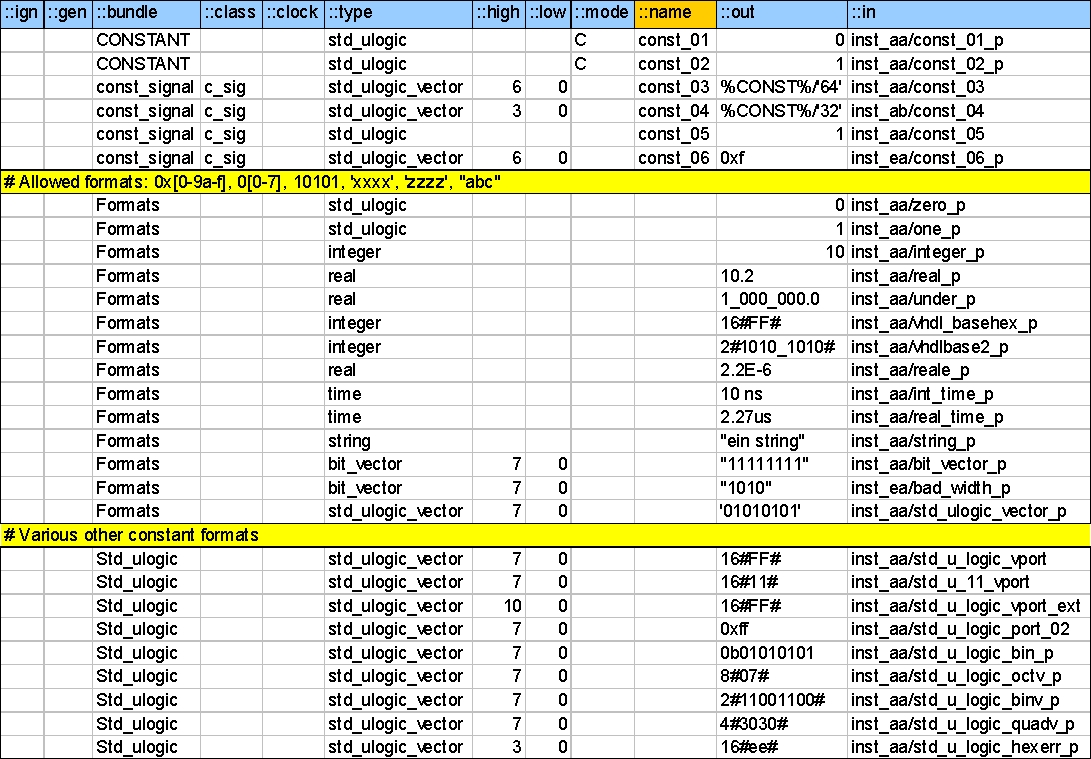
\includegraphics[scale=0.43]{images/mix_table1.jpg}\\
\newline
If the target language is VHDL, XXXXX\newline
MIX looks like in the following screenshot:\newline
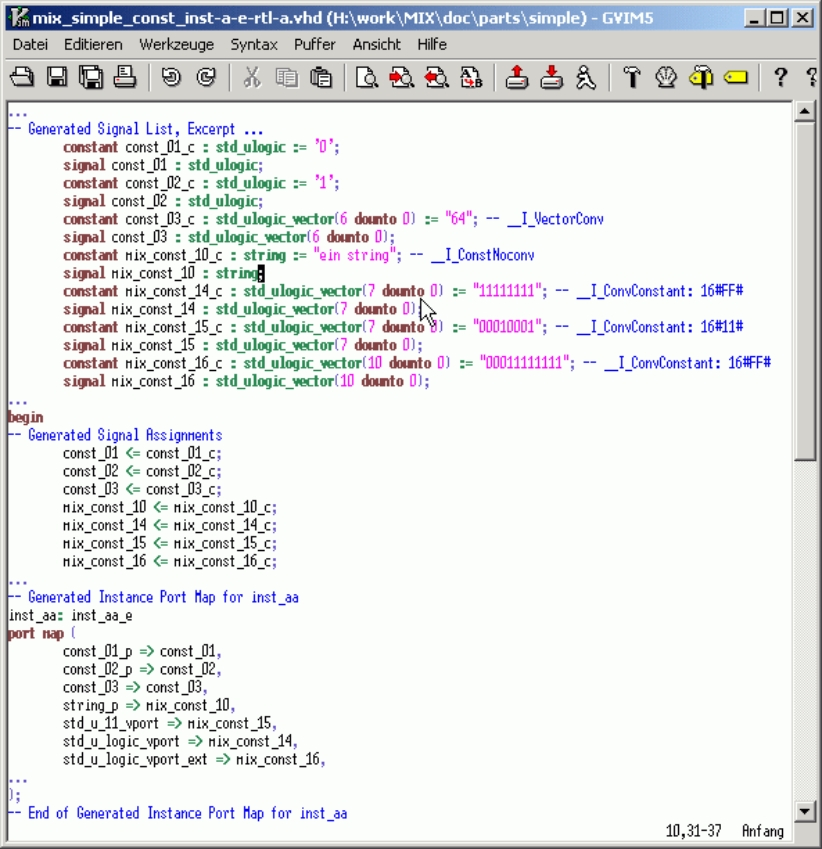
\includegraphics[scale=0.4]{images/mix_simple_inst.jpg}\\
Search for lines with \begin{tt}\_\_E\end{tt} in the comments to detect constants MIX was not able to translate properly. Verilog constant output is not very mature as of today.\newline

\subsubsection{Generics and Parameters}
Generics for entities are defined by a \begin{bf}G\end{bf} in the \begin{tt}::mode\end{tt} column. The \begin{tt}::name\end{tt} column defines the generics name. If the \begin{tt}::out\end{tt} column contains a string or a number, the value will be the default of this generic.\newline
A \begin{bf}P\end{bf} in the \begin{tt}::mode\end{tt} column marks parameters. The value given in the \begin{tt}::out\end{tt} column will be applied to the instances in the \begin{tt}::in\end{tt} column.\newline
If the \begin{tt}::name\end{tt} column is empty, MIX will assign a generated name. The HDL generic name is either the "port" name given in the \begin{tt}::in\end{tt} column or the \begin{tt}::name\end{tt}.\newline
A example description taken from a CONN sheet will create the following output in VHDL:\\
\begin{table}[htb]\begin{tabular}{|p{3cm}|p{2cm}|p{3cm}|p{2cm}|p{3cm}|}\hline
\begin{bf}::type\end{bf} & \begin{bf}::mode\end{bf} & \begin{bf}::name\end{bf} & \begin{bf}::out\end{bf} & \begin{bf}::in\end{bf}\\\hline
integer & G & generic\_a & 7 & g/generic\_a \\\hline
integer & P & parameter\_a & 16 & g/generic\_a \\\hline
string & G & generic\_b & "text" & g/generic\_b \\\hline
string & P & parameter\_b & "text" & g/generic\_b \\\hline
\end{tabular}\end{table}\\
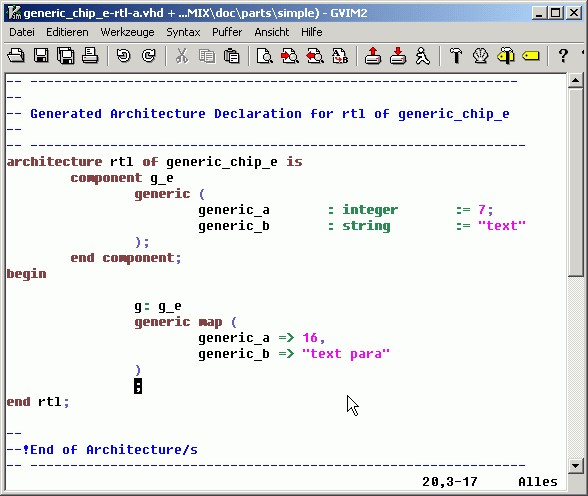
\includegraphics[scale=0.8]{images/mix_generic_chip.jpg}\\

\subsection{Simple text macros}
Text marked with with a \% on both sides is subject to be replaced, if a macro or a postfix of that name is defined. See the table of predefined macros. Additionally the contents of the input table can be referenced like \%::column\_head\%. If no suitable text macro is found, the text will be left as is.\newline
The text macro replacement does not operate recursively in general.\newline
\newline
Please consider that some text macros are used internally and some have a special meaning, too. E.g. the pseudo signals \%OPEN\% and \%LOW\_BUS\%.

\subsection{Predefined and user macros}
The following table contains a list of predefined macros. Some of them are defined at run time (e.g. the current date), some are for internal purposes only. macros marked with a yes in the "User" column can be set freely by the user on the command line or in the \begin{tt}mix.cfg\end{tt} configuration file.\newline

\begin{supertabular}{|p{45mm}|p{6cm}|p{3cm}|l|}\hline
\begin{bf}Macro Name\end{bf}&\begin{bf}Default Value\end{bf}&\begin{bf}Description\end{bf}&\begin{bf}User\end{bf}\\\hline
\%0\% & mix\_0.pl & Program name & \begin{it}run time\end{it} \\\hline
\%ARGV\% & K:$\backslash$Projects$\backslash$MIX$\backslash$PROG $\backslash$mix\_0.pl -listconf & Program arguments & \begin{it}run time\end{it} \\\hline
\%BUFFER\% & buffer & & yes \\\hline
\%BUS\_TYPE\% & std\_ulogic\_vector & & yes \\\hline
\%CONST\% & \_\_CONST\_\_ & & yes\\\hline
\%DATE\% & Mon Jun 30 16:22:41 2003-06-30 & Current date & \begin{it}run time\end{it} \\\hline
\%DEFAULT\_MODE\% & S & Signal default mode & yes \\\hline
\%EMPTY\% & & Empty string & yes \\\hline
\%GENERIC\% & \_\_GENERIC\_\_ & & - \\\hline
\%H\% & \$ & internal & - \\\hline
\%HIGH\% & mix\_logic1 & Name of logic high value & yes \\\hline
\%HIGH\_BUS\% & mix\_logic1\_bus & Name of logic high value bus & yes \\\hline
\%HOME\% & H:$\backslash$ & & - \\\hline
\%IOCELL\_SELECT\_ PORT\% & select & & yes \\\hline
\%IOCELL\_TYPE\% & \_\_E\_DEFAULT\_IOCELL\_\_ & & - \\\hline
\%IOCR\% & $\backslash$n & & - \\\hline
\%LANGUAGE\% & vhdl & & yes \\\hline
\%LOW\% & mix\_logic0 & & yes \\\hline
\%LOW\_BUS\% & mix\_logic0\_bus & & yes \\\hline
\%NULL\% & 0 & & - \\\hline
\%OPEN\% & open & & - \\\hline
\%PAD\_CLASS\% & PAD & & yes \\\hline
\%PAD\_TYPE\% & \_\_E\_DEFAULT\_PAD\_\_ & & - \\\hline
\%PARAMETER\% & \_\_PARAMETER\_\_ & & - \\\hline
\%PROJECT\% & NO\_PROJECT\_SET & & yes \\\hline
\%SIGNAL\% & std\_logic & & yes \\\hline
\%SPACE\% & & & yes \\\hline
\%TAB\% & $\backslash$t & & - \\\hline
\%TBD\% & \_\_W\_TO\_BE\_DEFINED & & - \\\hline
\%TOP\% & \_\_TOP\_\_ & & yes \\\hline
\%UNDEF\% & ERROR\_UNDEF & & - \\\hline
\%UNDEF\_1\% & ERROR\_UNDEF\_1 & & - \\\hline
\%UNDEF\_2\% & ERROR\_UNDEF\_2 & & - \\\hline
\%UNDEF\_3\% & ERROR\_UNDEF\_3 & & - \\\hline
\%UNDEF\_4\% & ERROR\_UNDEF\_4 & & - \\\hline
\%USER\% & wig & & \begin{it}run time\end{it}\\\hline
\%VERILOG\_TIMESC ALE\% & 'timescale 1ns / 1ns; & & yes \\\hline
\%VERSION\% & Revision 1.12 & & - \\\hline
\%VHDL\_NOPROJ\% & -- No project specific VHDL libraries & & - \\\hline
\%VHDL\_USE\% & -- No project specific VHDL libraries & & yes \\\hline
\%VHDL\_USE\_ARCH\% & \%VHDL\_USE\_DEFAULT\%    \%VHDL\_USE\% & & yes \\\hline
\%VHDL\_USE\_CONF\% & \%VHDL\_USE\_DEFAULT\%    \%VHDL\_USE\% & & yes \\\hline
\%VHDL\_USE\_DEFA ULT\% & library IEEE;  use IEEE.std\_logic\_1164.all & & yes \\\hline
\%VHDL\_USE\_ENTI TY\% & \%VHDL\_USE\_DEFAULT\%    \%VHDL\_USE\% & & yes \\\hline
\end{supertabular}
\newline
\newline
The default values can be changed by using\newline
\hspace*{20mm}\begin{tt}-conf macro.\%THIS\_MACRO\%=my\_value\end{tt}\newline
command line switch. New macros can be defined the same way.\newline
Alternatively a line like\newline
\hspace*{20mm}\begin{tt}MIXCFG macro.\%THIS\_MACRO\% my\_value\end{tt}\newline
to the mix.cfg configuration file will achieve the same result.\newline

\section{CONN sheet macros}
To simplify the wiring of standard interfaces, MIX provides the connection macro facility. The connection macros are entered just like any other connection, but are marked by MH, MD and MX in the ::gen column. MH is the macro header line, which has to be followed by one to many MD macro definition row. The first non-comment line without a MD tag stops the macro definition.\newline
The tag MX marks lines subject to be macro expanded. The macro expansion takes place after the initial tables were parsed.\newline
You can define simple, one-letter variabes in the macro cells. Any text in ::ign, ::gen, ::comment and ::descr cells of a MH and MX row will not be subject to matching and evaluation, but be ignored. Apart from that the column names have no special meaning.\newline
\newline
A simple example will illustrate the connection macro usage.\newline
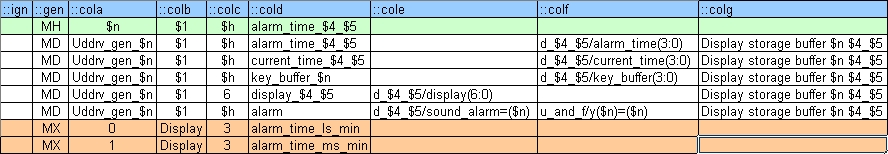
\includegraphics[scale=0.54]{images/macro.jpg}\\
Here the macro header MH defines the variables \$n, \$1, \$h, \$4 and \$5. The MIX parser extracts the MH row and accompanying MD rows (five lines here) from the table. In a second run each MX row will trigger a match operation against all MH definitions. MX and MH are a match, if each cell defined in the MH row has a matching counterpart in the MX row. Variables in the MH cells are considered to match any string ( .+ in perl regular expression syntax). Thus the first MX line matches the MH lines here. The variables defined in the MH cells are assigned the matching values from the MX line. E.g. \$n will be 0 for the first MX, 1 for the second. The variable \$4 is assignd ls, \$5 is min.\newline
\newline
If MX and MH match, the accompanying MD lines are executed. Variables are replaced by the value they are assigned too, currently. Here the first MX will result in the following table to be generated:\newline
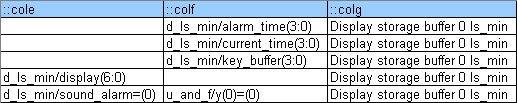
\includegraphics[scale=0.66]{images/macro_out.jpg}\\
The ::gen column is set to G\_MX after evaluation. Empty cells in MD lines are filled with the value given by MX, if any.\newline
\newline
Please see the contrib directory for commonly available connection macros (t.b.d.).

%not text macros, but MH, MD and MX generators:\newline
%\newline
%\hspace*{2mm}MH: Macro header: needs to match against the MX line (\$X defines variables)\newline
%\hspace*{2mm}MD: Body of macro. Will be inserted after variable replacement.\newline
%\hspace*{2mm}MX: Triggers macro expansion. Will be matched against all MH lines known.\newline
%\hspace*{12mm}Defines variable values.\newline

\section{Generator statements}
\subsection{Hierachy Generator Operators}
Another powerfull feature of MIX are the generator statements. The generators are applied after initial tool setup and connection macro evaluation, first the hierachy generators, then the connection generators.\newline
\newline
Generators are defined in the ::gen column. Basically three types are available:\newline
\begin{itemize}
\item{ Constructor generators: \$i(N..M)}
\item{ Match generator: /match\_expression/}
\item{ Bounded match generator: \$i(N..M),/match\_expression/}
\end{itemize}
match\_expression is like perl(1) regular expressions, but with some extensions and specials.\newline

\subsubsection{Constructor Generator statement}
MIX takes the variable and the range definied in ::gen and evaluates the rest of the row for each value in the range. Currently only one variable is allowed and the range has to be of form (N..M).\newline
\newline
A simple example illustrates the usage:\\
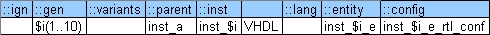
\includegraphics[scale=0.8]{images/gen_it.jpg}\\
will give ten instances from inst\_1 to inst\_10, each being a submodule of inst\_a with each having a entity inst\_1\_e to inst\_10\_e, dito. for the configuration. Simple arithmetic can be applied to derive values from the run time parameter \$i.\newline
Constructor's will yield new instances. An instance name has to be given in the ::inst column.\newline

\subsubsection{Match generator}
For each instance defined up to now, match\_expression is evaluated. If this yields true, the line is executed. Parts of the expression in parantheses are used to set the variables \$1, \$2, ... accordingly. See the perl regular expression man page perlre(1) for more details. This variables can be used in the other cells. Simple arithmetic is possible, e.g. {\$i + 1} or {\$1 * 2}.\newline
A match generator will yield new instances only if the name in the ::inst column is set to a value different from the matching instance.\newline
\newline
Example:\newline
\newline
XXX t.b.d.\newline

\subsubsection{Bounded match generator}
By adding a run variable and a range \$i(N..M), match generators can be restricted to only apply if the variable \$i is within the range. \$i has to be defined in match\_expression and will match any number.\newline
\newline
In opposite to the constructor generator, MIX will not evaluate all possible values for \$i, but only make sure \$i stays within the bounds of the range.\newline
\newline
Example:\newline
\newline
XXX t.b.d.\newline

\subsubsection{Advanced features of the match generators}
The match expression can contain references to all fields of the to match object with the\newline
::NAME\_OF\_COL=string(match):: reference.\newline
\newline
E.g. the connection generator\newline
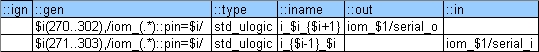
\includegraphics[scale=0.80]{images/gen_2.jpg}\\
will wire all instances iom\_.* having a property ::pin in the given range with a newly defined signal i\_N\_{N+1}. iom\_foo with ::pin = 270 port serial\_o will drive the signal i\_270\_271, the instance iom\_bar with ::pin = 271 is connected to the signal i\_270\_271 to it's port serial\_i by the next line. for instance iom\_foo only the first line matches, thus that module will net get a connection to serial\_i by these generator lines.\newline
\newline
A trainling :: can be omitted. If two propertied are to be matched, this will look like\newline
\hspace*{10mm}/::prop1=(.*)::::prop2=string(match?)/

\subsubsection{Additional Information}
Match generators work the same way on the CONN sheets. By default the match expression will match against all defined instances, not connections.\newline
To make a match expression iterate over all connection, prefix the whole expression by the CONN: keyword.\newline
\newline
Please have a look into the distributed howto.xls and the macro.xls in the test case directory t to see more examples.

\section{IO sheet}
A third category of input specification is the IO sheet. The contents of the IO sheet is parsed and translated into instances of io cell blocks and pad cells and connections of the io logic with the design core logic.\\
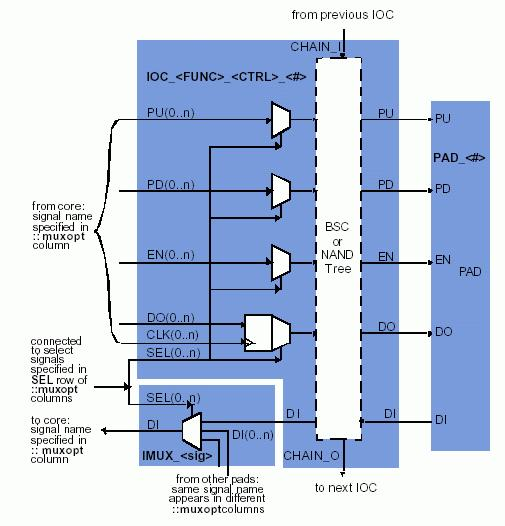
\includegraphics[scale=0.7]{images/mix_iocell.jpg}\\
Image 3: IO Cell and Pad Layout\newline
The IO sheet is a simple way to specify the connections of the IO cell to the design core logic. MIX will derive the connections of the DI(0..n), DO(0..n), PU(0..n), PD(0..n), EN(0..n) and the accompanying select lines. MIX will not add special purpose connections and the IO cell to Pad cell connections. This should be done by using the macro and generator statements in the CONN sheets.\newline
A simple example illustrates the various input fields and their usage.\\
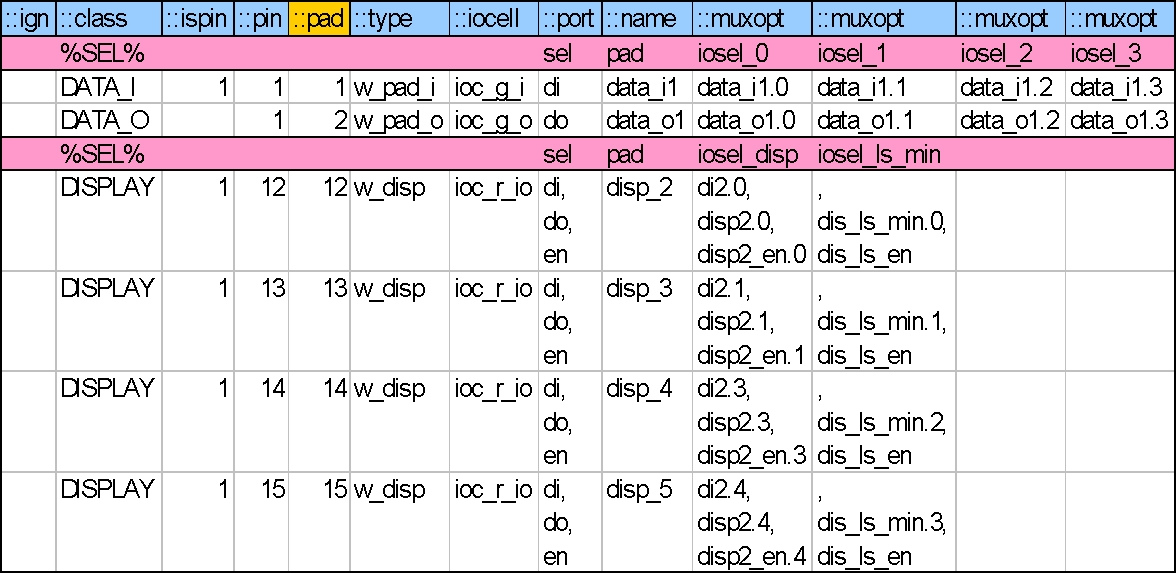
\includegraphics[scale=0.4]{images/mix_io_sheet.jpg}\\
\subsection{IO sheet column header}
The IO sheet starts with the usual header line, defining mandatory and optional columns:\newline
\hspace*{4mm}-\hspace*{4mm}\begin{tt}::ign\end{tt}\hspace*{9mm}A \begin{tt}\#\end{tt} marks a comment line. Has to be first column. Optional.\newline
\hspace*{4mm}-\hspace*{4mm}\begin{tt}::class\end{tt}\hspace*{4mm}The class name is forwarded to the \begin{tt}::class\end{tt} field of the CONN sheet. (opt.)\newline
\hspace*{4mm}-\hspace*{4mm}\begin{tt}::ispin\end{tt}\hspace*{4mm}Set to one it this pad is actually bonded (ignored by MIX).\newline
\hspace*{4mm}-\hspace*{4mm}\begin{tt}::pin\end{tt}\hspace*{8mm}Number or name of the pin. (ignored by MIX)\newline
\hspace*{4mm}-\hspace*{4mm}\begin{tt}::pad\end{tt}\hspace*{8mm}The primary key of the IO sheet. Has to an integer value. The pad\newline
\hspace*{32mm}numbers do not have to be consecutive. Mandatory column.\newline
\hspace*{4mm}-\hspace*{4mm}\begin{tt}::type\end{tt}\hspace*{7mm}Defines the entity of the generated pad cell.\newline
\hspace*{4mm}-\hspace*{4mm}\begin{tt}::iocell\end{tt}\hspace*{3mm}Defines name and entitiy of the generated io cell\newline
\hspace*{4mm}-\hspace*{4mm}\begin{tt}::port\end{tt}\hspace*{7mm}Define the io cell port name towards to the core logic. Port\newline
\hspace*{32mm} names are separated by , and/or <Alt><CR>.\newline
\hspace*{4mm}-\hspace*{4mm}\begin{tt}::name\end{tt}\hspace*{8mm}pad name\newline
\hspace*{4mm}-\hspace*{4mm}\begin{tt}::muxopt\end{tt}\hspace*{4mm}Connection matrix of io cell ports to core logic. Signals are separated\newline
\hspace*{33mm}by , and/or <Alt>-<CR>. Signals may be single bits or a one bit bus\newline
\hspace*{33mm}slice. Type \begin{tt}core\_sig.N\end{tt} or \begin{tt}core\_sig(N)\end{tt} for bit N of the core signale\newline
\hspace*{33mm}\begin{tt}core\_sig\end{tt}.\begin{tt}::muxopt\end{tt} is allowed to appear several times. The number of\newline
\hspace*{33mm}signals and the order matches the port names in the ::port field.\newline

\subsection{IO sheet \%SEL\% rows}
The rows with the key \begin{tt}\%SEL\%\end{tt} in the \begin{tt}::class\end{tt} field define the wiring of the IO cells multiplexer select lines. The  name in the \begin{tt}::port\end{tt} field defined the io cell port to connect to. The \begin{tt}::name\end{tt} field is ignored. The signal names listed in the \begin{tt}::muxopt\end{tt} columns are connected from the designs core with the appropriate slice of the io cell multiplexer select lines (one hot select lines). The leftmost \begin{tt}::muxopt\end{tt} connects to bit 0, the next to bit 1 and so forth. \begin{tt}core\_sel.N\end{tt} or \begin{tt}core\_cel(N)\end{tt}. can be used to wire select buses. The number of non-empty consecutive \begin{tt}::muxopt\end{tt} fields also define the width of the multiplexer. The actual multiplexer width is stored in the \begin{tt}\%::\_muxwidth\_\%\end{tt} field.\newline
The given values for the select lines are valid until the last row or another \begin{tt}\%SEL\%\end{tt} line is found.\newline
\begin{tt}\%NOSEL\%\end{tt} will stop usage of in/out multiplexer and select lines.\newline
Setting the configuration switch "\begin{tt}iocell.select\end{tt}" to "\begin{tt}bus\end{tt}" changes from a one-hot architecture to a select bus architecture. The select bus name is take in the leftmost \begin{tt}::muxopt\end{tt} column, an appropriate width is calculated by the number of defined \begin{tt}::muxopt\end{tt} columns.\newline

\subsection{IO sheet pad rows}
All other rows make up the connection matrix. For each row an io cell is instantiated. By default this io cell's name is composed by the type listed in the \begin{tt}::type\end{tt} field with the \begin{tt}::pad\end{tt} number attached, separated by a \begin{tt}\_\end{tt}.\newline
Secondly a pad cell is instantiated. By default this pad cell's name is composed from the prefix \begin{tt}pad\_\end{tt} and the pad number as given in the \begin{tt}::pad\end{tt} field. The default naming for both io cell and pad is given by the configuration variables\newline
\hspace*{20mm}\begin{tt}pad.name = \%PREFIX\_PAD\_GEN\%\%::pad\%\end{tt}\newline
\hspace*{20mm}\begin{tt}iocell.name = \%::iocell\%\_\%::pad\%\end{tt}\newline
You can leave unused \begin{tt}::muxopt\end{tt} columns empty. Then MIX will reduce the number of select lines accordingly.

\subsection{IO cell and Pad connections}
MIX IO sheet parser connects the IO cell internal interface towards the design core logic, only. Connections between pad and io cell need to be defined explicitely, usually be means of \begin{tt}::gen\end{tt} match operators.\newline
Additonal wires for NAND tree or boundary scan are specified the same way.Signal busses need to be defined properly, esp. the width and type. MIX will derive these properties from the definition.\newline
The generated pad and iocells need to be linked into the design hierarchy properly, e.g. by adding \begin{tt}::gen\end{tt} match operators in the \begin{tt}HIER\end{tt} sheet.\\
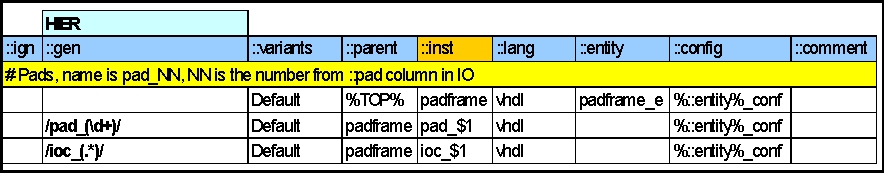
\includegraphics[scale=0.40]{images/mix_hier_sheet.jpg}\\
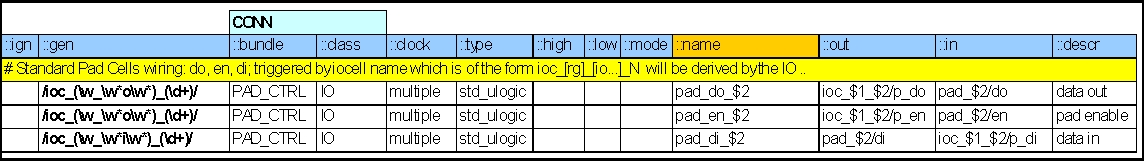
\includegraphics[scale=0.45]{images/mix_conn_sheet.jpg}

\subsection{IO Parser global configuration}
Some global configuration are available to tailor the IO sheet parser behaviour:\newline
\begin{tabular}{|p{4cm}|p{9cm}|}\hline
\begin{tt}iocell.name\end{tt} & Rule determines naming of the io cell instances. Default "\begin{tt}\%::iocell\_\%::pad\%\end{tt}" \\\hline
\begin{tt}iocell.auto\end{tt} & If set to "\begin{tt}bus\end{tt}", create busses as needed. Otherwise MIX relies on appropriate definition of busses by the CONN sheets. \\\hline
\begin{tt}iocell.bus\end{tt} & If \begin{tt}iocell.auto\end{tt} is set to bus, MIX will attach the keyword listed here (\begin{tt}\_vector\end{tt}) to signal type definitions. \\\hline
\begin{tt}iocell.defaultdir\end{tt} & Defines default iocell port direction. Default: \begin{tt}in\end{tt} \\\hline
\begin{tt}iocell.in\end{tt} & comma and/or white-space separated list of in ports Default: \begin{tt}do, en, pu, pd, xout\end{tt} \\\hline
\begin{tt}iocell.out\end{tt} & list of io-cells out ports Default: \begin{tt}di, xin\end{tt}\\\hline
\begin{tt}iocell.select\end{tt} & List of keywords defining the select multiplexer connections: \begin{tt}onehot\end{tt} -$>$ use one hot architecture for select lines, \begin{tt}bus\end{tt} -$>$ use select line bus, \begin{tt}auto\end{tt} -$>$ calculate width of select bus or one-hot based on \begin{tt}\%SEL\%\end{tt} width; Default: \begin{tt}onehot,auto\end{tt}\\\hline
\begin{tt}pad.name\end{tt} & Rule determines the naming of the pad instances. Default: "\begin{tt}\%PREFIX\_PAD\_GEN\%\%::pad\%\end{tt}" \\\hline
\end{tabular}

\section{I2C sheet}
The I2C sheet is one more category of input specification. It's content describes I2C Register's 

\section{VI2C sheet}

\section{Alarm clock example}

\section{Alarm clock example}

\section{MIX converter man page}

\subsection{Synopsis}

\subsection{Command line switches}
\begin{tt}-out OUTPUTFILE.ext\end{tt}\newline
\hspace*{15mm}defines output filename and type\newline
\begin{tt}-outenty OUT-e.vhd|ENTY|COMB\end{tt}\newline
\hspace*{15mm}Write all entities into OUT-e.vhd.\newline
\hspace*{15mm}If argument is ENTY, each entity will be written\newline
\hspace*{15mm}into a file called entityname-e.vhd.. (The exact\newline
\hspace*{15mm}naming depends on changeable rules).\newline
\hspace*{15mm}If argument is COMB, entity, architecture and configuration\newline
\hspace*{15mm}will all be written into one file called entityname.vhd\newline
\begin{tt}-outarch OUT-rtl-a.vhd|ARCH|COMB\end{tt}\newline
\hspace*{15mm}See description of outenty option.\newline
\begin{tt}-outconf OUT-c.vhd|CONF|COMB\end{tt}\newline
\hspace*{15mm}See description of outenty option.\newline
\begin{tt}-combine\end{tt}\newline
\hspace*{15mm}write entity, architecture and configuration into one file for \newline
\hspace*{15mm}each entity. Shortcut for setting -out[enty|arch|conf] to COMB\newline
\hspace*{15mm}individually.\newline
\begin{tt}-dir DIRECTORY\end{tt}\newline
\hspace*{15mm}write intermediate, internal and backend data into the given\newline
\hspace*{15mm}DIRECTORY. By default MIX writes to the current working directory\newline
\begin{tt}-top TOPCELL\end{tt}\newline
\hspace*{15mm}use TOPCELL as top. Default is TESTBENCH or daughter of TESTBENCH.\newline
\begin{tt}-adump\end{tt}\newline
\hspace*{15mm}dump internal data in ASCII format, too\newline
\hspace*{15mm}(debugging, use with small data set).\newline
\begin{tt}-variant VAR1\end{tt}
\hspace*{15mm}Select VAR1 from the HIER worksheet.\newline
\begin{tt}-conf key.key.key=value\end{tt}\newline
\hspace*{15mm}Overload \$EH{key}{key}{key} with value or add a\newline
\hspace*{15mm}new configuration variable.\newline
\begin{tt}-listconf\end{tt}\newline
\hspace*{15mm}Print out all available/predefined configurations options\newline
\begin{tt}-delta\end{tt}\newline
\hspace*{15mm}Output will be compared against previous runs.\newline
\begin{tt}-sheet SHEET=MATCH\end{tt}\newline
\hspace*{15mm}SHEET can be one of "hier", "conn", "vi2c". MATCH is\newline
\hspace*{15mm}a perl regular expression.\newline
\begin{tt}-strip\end{tt}\newline
\hspace*{15mm}Remove old and diff sheets. These sheets are named with "O\_" or "DIFF".\newline
\newline
\# Add your options here ....\newline
\newline
\newline
"Standard" options:\newline
\hspace*{15mm}\begin{tt}my @stdopts = qw(help|h! verbose|v! quiet|q! nobanner!  debug:i\end{tt}\newline
\hspace*{20mm}\begin{tt}makeopts=s@ gmakeopts=s@);\end{tt}\newline
Caveat: the -h option will not work on MS-Windows

\subsection{Runtime options and configuration}
Runtime configuration is controlled by (increasing precedence):
\begin{itemize}
\item built-in default values
\item \begin{tt}mix.cfg\end{tt} files, if found \begin{tt}\$HOME\end{tt}, \begin{tt}\$PROJECT\end{tt} and/or in current directory. Format is: \begin{tt}MIXCFG name.of.conf\end{tt} \begin{it}value\end{it}
\item CONF sheet found in input xls files
\item command line switch: \begin{tt}-conf foo.bar=\end{tt}\begin{it}value\end{it}
\item dedicated command line options
\end{itemize}
MIX reads in \begin{tt}mix.cfg\end{tt} configuration files in the following locations:
\begin{enumerate}
\item{\begin{tt}\$ENV\{HOME\end{tt}\}\newline
"\begin{tt}HOMEDRIVE\end{tt}", "\begin{tt}HOMEPATH\end{tt}", "\begin{tt}USERPROFILE\end{tt}" or "\begin{tt}C:$\backslash$\end{tt}"\newline
(only from the first matching location)}\newline
\item{\begin{tt}\$ENV\{PROJECT\}\end{tt}}
\item{"\begin{tt}.\end{tt}" (cwd)}
\end{enumerate}
Order: \begin{tt}HOME\end{tt} / \begin{tt}HOME\end{tt} / \begin{tt}cwd()\end{tt} / \begin{tt}-conf\end{tt} (last wins)

\subsection{Misc features}

\subsubsection{-delta mode}
Do not change output files, but report number of changes. Adds extra sheets \begin{tt}DIFF\_CONN\end{tt} and \begin{tt}DIFF\_HIER\end{tt} (and old versions of them) to the intermediate output. The \begin{tt}FOO.pld\end{tt} internal output gets overwritten, though. All messages are appended to \begin{tt}mix\_0.pl\end{tt}\newline
If a new HDL-file needs to be created by the changes, the -delta mode is not be applied for that file, but it is generated as new. If you never have written a \begin{tt}FOO-mixed.xls\end{tt} intermediate output, there is no \begin{tt}HIER\end{tt} or \begin{tt}CONN\end{tt} sheet generated.\newline
By adding the following two lines to your configuration (e.g. \begin{tt}./mix.cfg\end{tt}), delta mode will be the default:\newline
\newline
\begin{tt}MIXCFG output.generate.delta 1\end{tt}\newline
\begin{tt}MIXCFG output.delta sort,remove\end{tt}\newline
\newline
See the configuration option description for more details.\newline
\newline
\hspace*{10mm}\begin{tt}-nodelta\end{tt} switches delta mode off, then.\newline

\subsubsection{Imtermediate Excel Sheet}
Format of intermediate xls sheet will be kept as is as long as the number and order of columns is unchanged.\newline
MIX saves three old versions of the generated \begin{tt}HIER\end{tt} and \begin{tt}CONN\end{tt} sheets. The worksheets names are rotated by a trailing \begin{tt}\_\end{tt} and number.

\subsubsection{Output Redirection}
MIX writes all output into the current working directory. By using the\newline
\hspace*{20mm}\begin{tt}-dir DIRECTORY\end{tt}\newline
option, you can set the output directory for all intermediate, internal and HDL files to \begin{tt}DIRECTORY\end{tt}. Absolute path names defined by other options (e.g. -out) are not changed, though. If \begin{tt}DIRECTORY\end{tt} does not exist it will be created.
To have separate output directories, use the \begin{tt}mix.cfg\end{tt} file:\newline
\hspace*{20mm}\begin{tt}MIXCFG output.path HDLDIRS\end{tt}\newline
\hspace*{20mm}\begin{tt}MIXCFG internal.path MIXINTERNAL\end{tt}\newline
\hspace*{20mm}\begin{tt}MIXCFG intermediate MIXINTERMEDIATE\end{tt}\newline
writes internal, intermediate and HDL files to the given pathes. All directories have to exist and will not be created.

\section{Alarm clock example}
\subsection{Core logic}
\subsection{IO logic}
\section{Other examples}

\section{Known Bugs and limitations}
MS-Win/UNIX end-of-line issue:
Some EDA tools are not able to cope with the\newline
different end-of-line (CR vs LF/CR) of UNIX and MS-Windows. Use:\newline
\hspace*{15mm}\begin{tt}\$ module load freeware; recode "pc..lat1" *.vhd\end{tt}\newline
or (in MIX's Base directory):\newline
\hspace*{15mm}\begin{tt}\$ dos2unix.pl <filename>\end{tt}\newline
for Dos to Unix convertion and:\newline
\hspace*{15mm}\begin{tt}\$ unix2dos.pl <filename>\end{tt}\newline
for Unix to Dos convertion.

\section{Issue tracking: CADNET -> Issue tracking -> CAD Software -> MIX}
If you find unexpected or buggy behavior, please issue a trouble ticket. Don't forget to add a short description. The test case should contain all source files and also log files, the exact command line switches and configuration files applied.\newline
\begin{it}Please provide a comprehensive description of issues found including all required input data and command line switch to allow fast debugging and fixing.\end{it}

\section{Links}

\subsection{MIX paper and documentation}
EDP\_2003\_final\_030331.pdf\newline
MIX\_Specification.xls (see $\backslash$$\backslash$Galaxy$\backslash$Development$\backslash$PROJECTS$\backslash$MIX)\newline
MIX\_Intro.ppt (see $\backslash$$\backslash$Galaxy$\backslash$Development$\backslash$PROJECTS$\backslash$MIX\newline

\subsection{Micronas internal}
Micronas HDL coding guidelines.pdf

\subsection{Others}

\subsection{Resources}
\hspace*{10mm}Downloads for:\newline
\hspace*{20mm}- IO Examples\newline
\hspace*{20mm}- Standard bus examples\newline
\hspace*{20mm}- NAND Tree\newline
\hspace*{20mm}- BS example\newline
\hspace*{20mm}- miscellaneous useful macros\newline

\subsection{Used Software}
\hspace*{15mm}- Perl\newline
\hspace*{15mm}- Komodo\newline
\hspace*{15mm}- Vim\newline
\hspace*{15mm}- WinCVS\newline

\subsection{Release Notes}
\subsubsection{20030716}
\hspace*{10mm}see doc$\backslash$release\_20030716.txt

\subsubsection{20030709}
\hspace*{10mm}see doc$\backslash$release\_20030709.txt

\subsubsection{20030605}
\hspace*{10mm}See doc$\backslash$release\_20030605.txt

\end{document}
